%% JAIR Manuscript (acmart) - Clément Frassier
%% Apprentissage fédéré : principes et mise en œuvre
%% Détection du stress chez les infirmières hospitalières (Projet HEART)
%% Version synthétique (15 pages max) du rapport complet rapport_acc_nouveau_.tex

\documentclass{acmart}
\usepackage{amsmath, amssymb}
\usepackage{booktabs}
\usepackage{graphicx}
\usepackage{hyperref}
\usepackage{xcolor}
\usepackage{enumitem}
\setlist{itemsep=2pt, topsep=3pt}

%\setcopyright{cc}
%\acmDOI{10.1613/jair.1.xxxxx}

%\JAIRAE{Clément Frassier}
%\JAIRTrack{Applications}
%\acmVolume{4}
%\acmArticle{6}
%\acmMonth{8}
%\acmYear{2026}

\RequirePackage[
  datamodel=acmdatamodel,
  style=numeric,
  backend=biber,
  giveninits=true,
  uniquename=init
  ]{biblatex}

\renewcommand*{\bibopenbracket}{(}
\renewcommand*{\bibclosebracket}{)}

\addbibresource{sample-base.bib}

\begin{document}

\title[Hétérogénéité extrême en FL : le centralisé s'effondre aussi]{Quand l'hétérogénéité fait s'effondrer même le centralisé : une étude de cas en apprentissage fédéré pour la détection du stress infirmier \\ \large Version synthétique}

\author{Clément Frassier}
\orcid{0009-0000-0000-0000}
\email{clement.frassier@gmail.com}
\affiliation{%
  \institution{UKM / UEL}
  \city{Kuala Lumpur}
  \country{Malaysia}
}

\begin{abstract}
{\bf Background:}
Les données physiologiques collectées par bracelet connecté en milieu hospitalier
constituent des données de santé à caractère personnel soumises au
RGPD~\cite{gdpr2016}. Les agréger sur un serveur central expose les patients et le
personnel à des risques majeurs de ré-identification, rendant les approches
centralisées classiques inadaptées à ce contexte.

{\bf Objectives:}
Nous visons à entraîner un modèle de détection automatique du stress sur des données
distribuées entre 15 infirmières, sans jamais transmettre ces données à un serveur
central, tout en fournissant une garantie formelle de confidentialité différentielle
et en produisant un modèle déployable sur bracelet embarqué (TinyML).

{\bf Methods:}
Nous proposons un pipeline d'apprentissage fédéré combinant FedProx ($\mu = 0{,}05$)
pour la hétérogénéité Non-IID, et DP-SGD via Opacus pour la confidentialité
différentielle $(\varepsilon, \delta)$-DP. Le modèle MLP Tiny (1~362 paramètres,
5,32~Ko) est entraîné sur 30 rounds de communication et quantifié dynamiquement en
INT8 pour le déploiement. Une recherche sur grille de 25 runs fédérés
(5 valeurs de $\sigma \in [0{,}6;\, 1{,}8]$, 5 graines indépendantes) mesure
empiriquement le compromis confidentialité/utilité, comparée à une baseline
centralisée non contrainte (même modèle, mêmes 5 graines, sans FL ni DP) qui sert de
plafond de référence théorique -- non déployable en pratique sur ce type de données
de santé au sens du RGPD, mais utile pour quantifier honnêtement le coût de la
confidentialité.

{\bf Results:}
Sur un test-set groupé (toutes infirmières confondues), le modèle fédéré atteint une
précision de $82{,}0 \pm 0{,}5\,\%$ en moyenne sur les 5 valeurs de $\sigma$, contre
$81{,}95 \pm 0{,}89\,\%$ pour le centralisé -- des précisions brutes statistiquement
indiscernables. Sur des métriques équilibrées par classe, le centralisé conserve un
avantage apparent ($57{,}8 \pm 1{,}2\,\%$ de balanced-accuracy contre $\approx 47{,}9\,\%$
pour le FL). Mais 11 des 15 infirmières ont un test-set mono-classe, où une prédiction
constante obtient mécaniquement $100\,\%$ -- ces clients dominent le résultat groupé et
en masquent la vraie signification. Restreinte aux 4 clients au test-set réellement
mixte, la mesure la plus honnête cliniquement, l'écart se réduit fortement
($45{,}7 \pm 1{,}5\,\%$ pour le centralisé contre $42{,}7 \pm 1{,}0\,\%$ pour le FL) et
le \textbf{centralisé lui-même s'effondre} : son AUC-ROC tombe à $0{,}267$ (sous le
niveau du hasard) et son seuil de décision optimal se replie sur la prédiction
constante, exactement la même signature d'absence de signal généralisable que celle
attribuée au FL seul dans une évaluation groupée naïve. Une ablation FedProx sans DP-SGD
confirme que la fédération (pas la confidentialité) explique l'essentiel de l'écart
résiduel, la confidentialité ajoutant un coût mesurable mais secondaire, plus visible sur
ces clients difficiles ($45{,}2\,\%$ sans DP contre $42{,}7\,\%$ avec DP) que sur la
métrique groupée. Deux architectures de personnalisation (FedPer, puis une combinaison
tête multi-couches + DP restreint à l'extracteur + SCAFFOLD, cette dernière explorée
\emph{hors contrainte de taille TinyML}, à titre de comparaison haute plutôt que de
cible de déploiement) réduisent cet écart de façon statistiquement significative sur
les clients difficiles ($48{,}4\,\%$ puis $59{,}9\,\%$ de balanced-accuracy) sans le
faire disparaître. Fait notable, un simple fine-tuning post-hoc de la seule tête de
classification sur le modèle FedProx+DP standard déjà entraîné ($55{,}9\,\%$) surpasse
même FedPer, sans architecture dédiée ni surcoût de déploiement -- le résultat le plus
directement actionnable de ce travail pour un déploiement réel restant, lui, entièrement
dans l'enveloppe TinyML.

{\bf Conclusions:}
Le résultat central de ce travail n'est pas que le FL coûte cher face au centralisé --
c'est que \textbf{l'hétérogénéité extrême entre infirmières limite la généralisation de
toute architecture testée}, centralisée comprise : sur les clients au profil
physiologique le plus atypique, même un modèle entraîné sans aucune contrainte de
confidentialité ni de décentralisation échoue à produire un signal exploitable. Le FL
n'ajoute qu'un désavantage marginal, mais réel et mesurable, par-dessus ce problème de
fond. Ceci reformule la question de recherche : il ne s'agit pas de départager FL et
centralisé sur la précision (le centralisé restant de toute façon juridiquement
inadapté à ce type de données de santé au regard du RGPD, ce qui fait du FL la seule
approche viable en pratique), mais de comprendre pourquoi l'hétérogénéité Non-IID casse
la généralisation et comment la personnalisation architecturale (FedPer, SCAFFOLD) peut
la réduire. Nos résultats quantifient honnêtement ce coût résiduel, montrent qu'il reste
stable quel que soit le niveau de confidentialité visé, et qu'il peut être
significativement atténué par une architecture personnalisée -- tout en conservant un
modèle déployable sur microcontrôleur (5,32~Ko).
\end{abstract}

\received{20 May 2026}
\received[accepted]{1 July 2026}

\maketitle

\section{Introduction}

L'apprentissage fédéré (FL) entraîne un modèle collaboratif sans que les données
locales des clients ne quittent jamais leur appareil~\cite{mcmahan2017communication} --
une réponse directe aux exigences de minimisation des données du RGPD
(Art.~5)~\cite{gdpr2016} et de l'HIPAA~\cite{hipaa1996} en contexte médical. Ce
travail s'ancre sur un cas d'usage du projet HEART\footnote{Health, Engineering, AI,
Responsibility and TinyML -- collaboration UKM / University of East London.} : la
détection automatique du stress de 15 infirmières hospitalières à partir de signaux
physiologiques (bracelet connecté).

Ce travail part d'une question de comparaison (le FL peut-il approcher un modèle
centralisé ?) mais aboutit à un résultat plus fondamental : \textbf{l'hétérogénéité
physiologique extrême entre infirmières limite la généralisation de toute
architecture testée, centralisée y comprise} (Section~\ref{sec:discussion}). Sur les
clients au profil le plus atypique, même un modèle sans aucune contrainte de
confidentialité ni de décentralisation échoue à produire un signal exploitable. Ceci
déplace la question de recherche : non plus départager FL et centralisé sur la
précision, mais comprendre pourquoi l'hétérogénéité Non-IID casse la généralisation et
dans quelle mesure la personnalisation architecturale (FedPer, SCAFFOLD) peut la
réduire.

\paragraph{Positionnement.} FedAvg~\cite{mcmahan2017communication} suppose des données
client quasi-IID ; FedProx~\cite{li2020fedprox} relâche cette hypothèse via un terme
proximal mais évalue généralement son gain sur une hétérogénéité \emph{simulée}
(partitions Dirichlet synthétiques). La littérature sur la personnalisation en FL
(FedPer~\cite{arivazhagan2019federated}, et les mécanismes de correction de dérive
comme SCAFFOLD~\cite{karimireddy2020scaffold}) démontre généralement un gain de
personnalisation \emph{relatif} au modèle global fédéré, sans le confronter à un
plafond centralisé sur la même hétérogénéité réelle. La contribution empirique de ce
travail se situe précisément là : sur un jeu de données à hétérogénéité \emph{naturelle}
et extrême (physiologie individuelle, pas une partition synthétique), nous montrons que
le plafond centralisé lui-même s'effondre sur les clients les plus atypiques -- un
angle moins documenté dans cette littérature, qui compare le plus souvent le FL à un
centralisé implicitement supposé fiable.

\section{Méthodologie}
\label{sec:method}

\paragraph{Cycle FL.} À chaque round $t$, le serveur diffuse les poids globaux
$\mathbf{w}^{(t)}$ ; chaque client entraîne localement puis renvoie ses poids mis à
jour, agrégés par une moyenne pondérée par taille de partition (FedAvg,
\cite{mcmahan2017communication}).

\paragraph{Jeu de données.} \textit{Dataset for Continuous Stress Monitoring of
Hospital Nurses}~\cite{nurse_stress_dataset} : 15 infirmières équipées d'un bracelet
Empatica~E4 (EDA, fréquence cardiaque, température, accélération triaxiale). Les
séries brutes sont converties en fenêtres glissantes (taille 60, pas 30, 50~\% de
recouvrement), chacune résumée par 4 statistiques (moyenne, écart-type, min, max) sur
6 signaux, soit 24 caractéristiques par fenêtre. Le label brut à trois niveaux (pas de
stress / stress faible / stress élevé) est binarisé (stress vs. non-stress) pour
correspondre à la question clinique d'alerte temps réel. Le split train/test est
\textbf{chronologique par client} (80/20) avec un \textbf{gap de 2 fenêtres} entre les
deux pour éliminer toute fuite due au recouvrement des fenêtres ; la standardisation
est calculée localement, sur le train uniquement. Au total : \textbf{383\,584
fenêtres} (306\,886 train / 76\,698 test), 86,0~\% de stress sur le test-set groupé.

\textbf{Point méthodologique central} : \textbf{11 des 15 clients ont un test-set
mono-classe} (une seule des deux classes présente, par construction du split
chronologique). Le modèle appris développe un biais fort vers la classe majoritaire
globale (stress) : ce biais produit une accuracy quasi-parfaite sur 10 de ces 11
clients, mais s'inverse sur le 11\textsuperscript{e} (client 3, seul mono-classe sur la
classe \emph{minoritaire} : accuracy $\approx0\,\%$ avec FL+DP). Seuls \textbf{4
clients} (4, 5, 8, 12) ont un test-set réellement mixte et portent un signal
informatif sur la généralisation du modèle. Conséquence : toute métrique groupée sur
15 clients est fortement déformée par ces clients triviaux -- ce travail rapporte donc
systématiquement la métrique groupée \emph{et} la métrique restreinte aux 4 clients
informatifs, la seconde étant la plus honnête cliniquement.

\paragraph{Modèle et quantification.} MLP Tiny à trois couches entièrement connectées
($24\to32\to16\to2$), \textbf{1\,362 paramètres} (5,32~Ko en FP32) -- taille
compatible avec la SRAM d'un microcontrôleur bas de gamme. Une quantification
dynamique post-entraînement (PyTorch, INT8) réduit la taille théorique à
$\approx1{,}4$~Ko (facteur $\times3{,}8$), évaluée à chaque round sans perturber
l'entraînement FP32 sous-jacent.

\paragraph{FedProx.} Face à la dérive de poids (\textit{client drift}) induite par le
Non-IID, chaque client résout $\min_{\mathbf w}\{F_k(\mathbf w) + \frac{\mu}{2}\|\mathbf
w - \mathbf w^{(t)}_{\text{global}}\|^2\}$~\cite{li2020fedprox}, avec $\mu=0{,}05$
(équilibre entre stabilité de FedAvg et adaptation locale).

\paragraph{Confidentialité différentielle.} DP-SGD~\cite{abadi2016deep} via
Opacus~\cite{opacus} : clipping des gradients par exemple à $C=1{,}0$, puis bruit
gaussien calibré par le multiplicateur $\sigma$. Le budget cumulé $\varepsilon$ est
suivi par l'accountant PRV d'Opacus, pour un $\delta=10^{-5}$ fixé.

\paragraph{Protocole expérimental.} Simulation Flower~\cite{beutel2020flower} des
15 clients sur un seul nœud. Grille complète : $\sigma\in\{0{,}6;0{,}8;1{,}0;1{,}4;1{,}8\}$
$\times$ 5 graines indépendantes (42, 123, 7, 2024, 31415) = \textbf{25 runs
fédérés}, 30 rounds, 2 époques locales/round. Une baseline centralisée (même modèle,
mêmes 5 graines, standardisation globale, sans FL ni DP) sert de plafond de référence.

\section{Résultats}
\label{sec:results}

\subsection{Comparaison globale FL vs Centralisé}

Chaque modèle final est évalué sur un test-set unique regroupant les 15 infirmières
(76\,698 fenêtres). Le Tableau~\ref{tab:main} moyenne les résultats sur les 5 valeurs
de $\sigma$ (FL) et les 5 graines (centralisé, sur les deux métriques).

\begin{table}[h!]
\centering
\small
\caption{Résultats globaux : FL (FedProx+DP, moyenne sur 5$\sigma\times$5 graines) vs
centralisé (5 graines).}
\label{tab:main}
\begin{tabular}{lcc}
\toprule
Métrique & FL (FedProx+DP) & Centralisé \\
\midrule
Précision (pooled, 15 clients)             & $82{,}0\pm0{,}5\,\%$  & $81{,}95\pm0{,}89\,\%$ \\
Balanced-accuracy (pooled)                  & $47{,}9\pm0{,}2\,\%$  & $57{,}84\pm1{,}16\,\%$ \\
\textbf{Balanced-accuracy (4 clients informatifs)}  & $\mathbf{42{,}73\pm0{,}97\,\%}$ & $\mathbf{45{,}73\pm1{,}54\,\%}$ \\
\textbf{AUC-ROC (4 clients informatifs)}    & $\mathbf{0{,}2047\pm0{,}0232}$ & $\mathbf{0{,}2669\pm0{,}0197}$ \\
Précision INT8 (interne)                    & $81{,}57\pm0{,}31\,\%$ & $81{,}43\pm1{,}13\,\%$ \\
Budget $\varepsilon$ ($\sigma=1{,}4$)       & $0{,}82\pm0{,}06$      & n/a \\
\bottomrule
\end{tabular}
\end{table}

La précision brute ne départage pas les deux conditions. Sur la métrique pooled, le
centralisé affiche un avantage apparent en balanced-accuracy -- mais cet avantage
\textbf{ne survit pas à la restriction aux 4 clients informatifs} : les deux
conditions y sont proches du hasard, et l'AUC du centralisé y est même
\emph{significativement inférieure à 0,5} (Section~\ref{sec:discussion}).

\subsection{Décomposition fédération vs confidentialité}

Une troisième condition (FedProx sans DP-SGD) isole la part de l'écart attribuable à
la confidentialité de celle attribuable à la fédération elle-même
(Tableau~\ref{tab:decomp}).

\begin{table}[h!]
\centering
\small
\caption{Centralisé / FL sans DP / FL+DP (balanced-accuracy, moyenne$\pm$écart-type).}
\label{tab:decomp}
\begin{tabular}{lccc}
\toprule
 & Centralisé & FL sans DP & FL + DP \\
\midrule
Pooled (15 clients)       & $57{,}84\pm1{,}16\,\%$ & $48{,}68\pm0{,}73\,\%$ & $47{,}83\pm0{,}35\,\%$ \\
\textbf{Informatifs (4/15)} & $\mathbf{45{,}73\pm1{,}54\,\%}$ & $\mathbf{45{,}18\pm2{,}38\,\%}$ & $\mathbf{42{,}73\pm0{,}97\,\%}$ \\
\bottomrule
\end{tabular}
\end{table}

Dans les deux lectures, l'essentiel de l'écart avec le centralisé est déjà présent
\emph{sans aucun DP-SGD} : la fédération domine largement le coût mesuré. Sur les
clients informatifs, le bruit DP-SGD ajoute un coût réel mais secondaire
(2,45 points), plus visible que sur la métrique pooled qui le dilue (moins d'un
point).

\subsection{Compromis confidentialité/utilité}

Le Tableau~\ref{tab:eps} détaille le budget $\varepsilon$ accumulé et la
balanced-accuracy groupée en fonction du niveau de bruit $\sigma$ (moyenne sur
5 graines, round 30).

\begin{table}[h!]
\centering
\small
\caption{Grille confidentialité/utilité (5 valeurs de $\sigma$, $\delta=10^{-5}$).}
\label{tab:eps}
\begin{tabular}{cccc}
\toprule
$\sigma$ & $\varepsilon$ (round 30) & Précision INT8 (interne) & Balanced-acc. (pooled) \\
\midrule
0,6 & $5{,}29\pm0{,}30$ & $81{,}70\pm0{,}15\,\%$ & $47{,}87\pm0{,}47\,\%$ \\
0,8 & $2{,}18\pm0{,}12$ & $81{,}60\pm0{,}26\,\%$ & $47{,}77\pm0{,}26\,\%$ \\
1,0 & $1{,}32\pm0{,}13$ & $81{,}43\pm0{,}46\,\%$ & $47{,}85\pm0{,}24\,\%$ \\
1,4 & $0{,}82\pm0{,}06$ & $81{,}50\pm0{,}43\,\%$ & $47{,}67\pm0{,}32\,\%$ \\
1,8 & $0{,}54\pm0{,}04$ & $81{,}60\pm0{,}17\,\%$ & $48{,}12\pm0{,}38\,\%$ \\
\bottomrule
\end{tabular}
\end{table}

$\varepsilon$ décroît de façon monotone et régulière avec $\sigma$, exactement comme
attendu mathématiquement. La précision INT8 et la balanced-accuracy groupée restent,
elles, quasiment constantes sur toute la plage ($47{,}9$ à $48{,}1\,\%$) : le compromis
confidentialité/utilité est empiriquement plat sur cette architecture et ce jeu de
données -- l'essentiel du coût lié à la confidentialité est déjà consommé au niveau de
bruit le plus faible testé. L'ablation de personnalisation locale (fine-tuning FedProx
en régime, sur les clients déjà vus) n'apporte par ailleurs qu'un gain marginal et
bruité (moins de 1,2 point en moyenne), suggérant que la personnalisation
\emph{architecturale} testée ci-dessous est une piste plus prometteuse que la simple
adaptation post-hoc en régime.

\subsection{Scénario du nouvel arrivant}

Un scénario de déploiement plus exigeant est celui d'une infirmière qui rejoint la
fédération \emph{après coup} : elle reçoit le modèle global déjà entraîné sur les
autres, sans jamais avoir contribué elle-même. Pour le simuler, le client 8 (test-set
non mono-classe, $36{,}0\,\%$ de stress) est totalement exclu de l'entraînement fédéré
(30 rounds, $\sigma=0{,}8$, 3 graines) : le modèle global final n'a donc jamais vu ses
données. Évalué directement (``jour 1'', zéro adaptation), il n'est qu'à peine au
niveau du hasard (balanced-accuracy $50{,}41\pm0{,}72\,\%$). Après seulement 8 époques
de fine-tuning local, la balanced-accuracy grimpe à $58{,}51\pm1{,}00\,\%$ (comparable
au centralisé) et le F1 macro quasiment double -- l'apport de l'adaptation locale se
révèle surtout pour un participant véritablement nouveau, pas pour un client déjà
intégré au cycle d'entraînement. Le rappel par classe révèle en outre, au jour 1, des
biais systématiques opposés selon le client (le modèle prédit presque exclusivement
``stress'' pour l'un, presque exclusivement ``non-stress'' pour l'autre) que la seule
balanced-accuracy proche de $50\,\%$ ne laisse pas deviner -- un résultat illustratif
(2 clients, 3 graines), pas une conclusion généralisable aux 15 infirmières.

\begin{table}[h!]
\centering
\small
\caption{Rappel par classe (seuil par défaut $0{,}5$), avant et après adaptation
locale -- plage min--max sur 3 graines.}
\label{tab:recall}
\begin{tabular}{lcc}
\toprule
Client / Condition & Rappel non-stress & Rappel stress \\
\midrule
Client 8, jour 1 (zéro adapt.)  & $0{,}00$--$2{,}48\,\%$   & $99{,}93$--$100{,}00\,\%$ \\
Client 8, après adapt. (8 ép.)  & $32{,}95$--$37{,}03\,\%$ & $81{,}17$--$86{,}28\,\%$ \\
Client 5, jour 1 (zéro adapt.)  & $68{,}00$--$96{,}00\,\%$ & $0{,}00$--$1{,}02\,\%$ \\
Client 5, après adapt. (8 ép.)  & $100{,}00\,\%^{a}$       & $3{,}13$--$19{,}66\,\%$ \\
\bottomrule
\end{tabular}

\vspace{2pt}
{\footnotesize $^{a}$Valeur exacte et identique sur les 3 graines (25/25 fenêtres
non-stress correctement classées) -- ce client ne compte que 25 fenêtres non-stress
au total, un dénominateur trop faible pour une estimation de rappel fiable sur cette
seule classe.}
\end{table}

Le Tableau~\ref{tab:recall} révèle deux échecs symétriques et opposés au jour 1 : le
client 8 prédit presque exclusivement ``stress'' (rappel stress $\approx100\,\%$,
rappel non-stress $\approx0\,\%$), tandis que le client 5 montre le biais inverse
(rappel non-stress $68$--$96\,\%$, rappel stress $\leq1{,}02\,\%$). Dans les deux cas,
la balanced-accuracy proche de $50\,\%$ du jour 1 cachait un biais systématique fort,
pas une absence de signal. L'adaptation locale corrige partiellement ces deux biais en
sens inverse, mais de façon incomplète pour le client 5 : le rappel stress ne remonte
qu'à $12{,}15\,\%$ en moyenne, cliniquement insuffisant pour un système d'alerte.

\paragraph{Diagnostic complémentaire (pas un protocole de déploiement) : calibration de
seuil post-adaptation.} Un balayage du seuil de décision sur les modèles adaptés révèle,
pour les deux clients, un potentiel de rappel supplémentaire non exploité au seuil par
défaut -- mais dans des directions opposées : le seuil optimal descend à $0{,}001$ pour
le client 5 (rappel stress porté à $42{,}53\,\%$ en moyenne) et monte à $0{,}950$ pour
le client 8 (rappel non-stress porté à $59{,}05$--$59{,}65\,\%$). Ce balayage sélectionne
le seuil qui maximise la métrique sur le test-set utilisé ensuite pour la rapporter :
c'est un outil de diagnostic légitime pour révéler un problème de calibration, pas un
protocole de déploiement validé -- le chiffre qui en résulte est une borne supérieure
optimiste, pas une performance attendue en production.

\paragraph{Le même scénario rejoué sous FedPer.} En l'absence de toute tête à hériter
(\texttt{fc3} n'étant jamais transmis), le ``jour 1'' FedPer utilise une tête vierge
initialisée aléatoirement, posée sur l'extracteur partagé. Cette source de bruit
supplémentaire, absente sous FedProx (où la tête héritée est déterministe à checkpoint
donné), produit une dispersion nettement plus large entre graines (client 8 :
balanced-accuracy $50{,}1$--$69{,}7\,\%$ ; client 5 : $5{,}3$--$50{,}0\,\%$). L'onboarding
(8 époques, tête seule, extracteur gelé) resserre fortement cette dispersion et porte le
rappel stress du client 5, au seuil par défaut, à $57{,}19\,\%$ en moyenne -- nettement
au-delà des $12{,}15\,\%$ obtenus par l'adaptation complète post-hoc de FedProx au même
seuil, et comparable au diagnostic de calibration de seuil ci-dessus, mais sans qu'aucun
seuil n'ait été recalibré.

\section{Discussion : pourquoi l'écart FL/centralisé n'est pas ce qu'il semble être}
\label{sec:discussion}

\subsection{Le centralisé s'effondre aussi sur les clients difficiles}
\label{subsec:collapse}

Restreinte aux 4 clients informatifs, la balanced-accuracy du \textbf{centralisé}
tombe à $45{,}73\pm1{,}54\,\%$ (à peine au-dessus du hasard) et son AUC-ROC à
$0{,}2669\pm0{,}0197$ -- \textbf{significativement inférieure à 0,5}, ce qui ne
signale pas une absence de signal mais un classement partiellement \emph{inversé} :
le modèle centralisé a appris une relation partiellement fausse sur ces clients. Le
balayage de seuil de décision le confirme : le seuil optimal du centralisé se replie
sur $0{,}001$ (prédire ``stress'' presque systématiquement), plafonnant à
\emph{exactement} $50{,}00\pm0{,}00\,\%$ -- identique dans sa forme à ce que ce travail
attribuait initialement au FL seul. Le FL+DP présente la même signature, un peu plus
marquée ($42{,}73\pm0{,}97\,\%$, AUC $0{,}2047\pm0{,}0232$, plafond
$46{,}98\pm1{,}28\,\%$).

Un test de Welch confirme que l'écart centralisé-vs-FL+DP est statistiquement
significatif sur ces 4 clients ($t=4{,}21$, $p=9{,}8\times10^{-3}$), mais que
l'écart centralisé-vs-FL-sans-DP ne l'est \emph{pas} ($t=0{,}44$, $p=0{,}68$) : sur ces
clients précis, c'est le bruit DP-SGD (pas la décentralisation) qui crée l'écart
mesurable avec le centralisé. Une vérification par taille d'effet (Cohen's $d=2{,}81$
contre $d=0{,}28$) et par sous-échantillonnage à puissance égale (significatif dans
99,7~\% de 2\,000 tirages) confirme que ce contraste n'est pas un artefact de taille
d'échantillon. \textbf{Limite à garder à l'esprit} : cette significativité repose sur
seulement 4 clients au test-set mixte -- un résultat solide sur \emph{ces}
infirmières, pas encore une généralisation démontrée à toute population hétérogène.

\textbf{Message central} : ce n'est pas ``le centralisé résout un problème que le FL
ne résout pas'', mais ``l'hétérogénéité extrême limite les deux architectures, le FL
n'ajoutant qu'un désavantage marginal par-dessus''. Une mitigation testée (loss
pondérée par classe) n'a apporté aucun gain mesurable ($-0{,}11$ point), cohérent avec
un problème qui émerge de l'\emph{agrégation} entre 15 clients hétérogènes, pas de la
fonction de perte locale.

\subsection{Personnalisation : FedPer et FedRep+SCAFFOLD}

Deux architectures, comparées au Tableau~\ref{tab:perso}, testent si la personnalisation peut réduire cet écart en évitant
d'agréger tout ou partie de la tête de classification :

\begin{itemize}
\item \textbf{FedPer}~\cite{arivazhagan2019federated} : l'extracteur (\texttt{fc1},
\texttt{fc2}) reste agrégé globalement, mais la couche de classification finale
(\texttt{fc3}, 34 paramètres) n'est jamais transmise ni agrégée -- chaque client garde
sa propre tête, entraînée en continu sur 30 rounds.
\item \textbf{FedRep+SCAFFOLD} (hors contrainte TinyML, contraintes de sécurité
seules) : tête multi-couches (306 paramètres), DP-SGD restreint au seul extracteur
partagé, et SCAFFOLD~\cite{karimireddy2020scaffold} remplace le terme proximal de
FedProx comme correction de dérive Non-IID sur l'extracteur.
\end{itemize}

\begin{table}[h!]
\centering
\small
\caption{FedProx+DP / FedPer / FedRep+SCAFFOLD (balanced-accuracy et AUC, moyenne sur
5$\sigma\times$5 graines).}
\label{tab:perso}
\begin{tabular}{lccc}
\toprule
 & FedProx+DP & FedPer & FedRep+SCAFFOLD \\
\midrule
Balanced-acc. (pooled)         & $47{,}86\pm0{,}35\,\%$ & $65{,}06\pm2{,}78\,\%$ & $\mathbf{77{,}57\pm0{,}72\,\%}$ \\
\textbf{Balanced-acc. (informatifs)} & $42{,}73\pm0{,}97\,\%$ & $48{,}44\pm3{,}65\,\%$ & $\mathbf{59{,}89\pm0{,}22\,\%}$ \\
\textbf{AUC-ROC (informatifs)} & $0{,}2047\pm0{,}0232$ & $0{,}4417\pm0{,}1022$ & $\mathbf{0{,}7269\pm0{,}0035}$ \\
\bottomrule
\end{tabular}
\end{table}

\begin{figure}[h!]
\centering
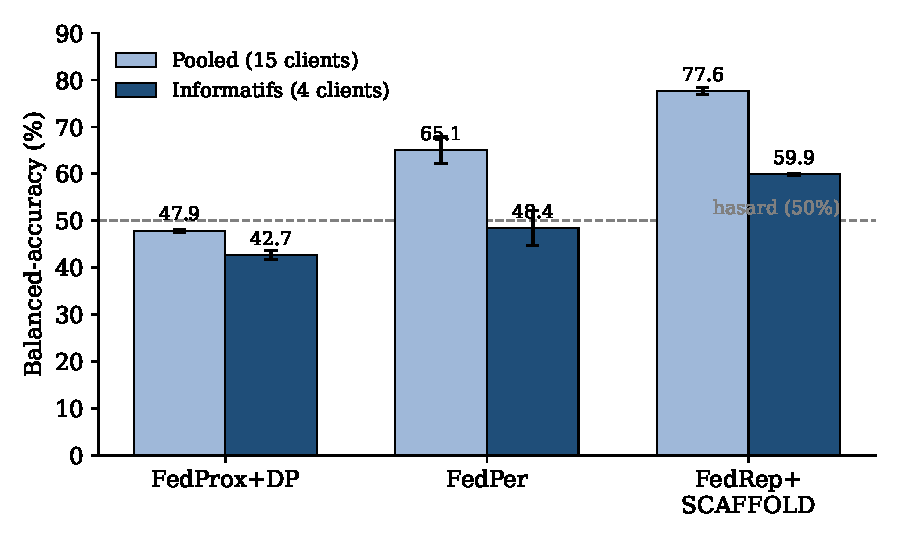
\includegraphics[width=0.8\linewidth]{fig_perso_comparison.pdf}
\caption{Balanced-accuracy des trois architectures, métrique pooled (15 clients)
contre métrique restreinte aux 4 clients informatifs -- l'écart entre les deux barres
de chaque paire est exactement le gonflement dû aux clients mono-classe
(Section~\ref{sec:method}).}
\label{fig:perso}
\end{figure}

Sur les clients informatifs, la hiérarchie FedProx+DP $<$ FedPer $<$ FedRep+SCAFFOLD
est statistiquement nette ($p<10^{-7}$ pour les trois comparaisons deux-à-deux) --
visible au premier coup d'œil sur la Figure~\ref{fig:perso}, où l'écart entre les deux
barres de chaque paire mesure directement combien la métrique pooled surestime la
performance réelle. Le
gain de FedPer (+5,7 points vs FedProx+DP) est solide mais nettement plus modeste que
le gonflement apparent sur la métrique pooled (+17,2 points) ; l'accuracy brute
progresse aussi, mais marginalement ($+0{,}95$ point, $p=0{,}04$). FedRep+SCAFFOLD va
plus loin (+17,2 points vs FedProx+DP sur les informatifs) et se montre nettement plus
stable (écart-type 0,22 contre 3,65 pour FedPer), au prix d'un coût de calcul
$\approx5\times$ supérieur et d'un facteur de confusion non résolu (tête à 2 couches
\emph{et} SCAFFOLD changent simultanément par rapport à FedPer).

\textbf{FedPer et FedProx diffèrent sur deux axes} : la durée de personnalisation
(30 rounds continus vs 8 époques de fine-tuning post-hoc) et la granularité (tête
seule vs réseau entier). Un test dédié, isolant ces deux facteurs à partir du même
checkpoint FedProx+DP et avec fine-tuning re-seedé (5 graines, test $t$ apparié),
montre que la \textbf{granularité domine largement} ($+7{,}4$ points à 8 époques,
$+6{,}5$ points à 30 époques, $p<0{,}03$) : personnaliser uniquement la tête surpasse
nettement le fine-tuning du réseau entier. La \textbf{durée compte aussi, mais
beaucoup plus modestement} ($+1$ à $+2$ points, $p<0{,}02$). Fait notable, un simple
fine-tuning de la tête seule sur le checkpoint FedProx+DP standard déjà entraîné
atteint $55{,}88\pm2{,}35\,\%$ -- \textbf{davantage que FedPer lui-même}, sans
architecture dédiée ni contrainte de déploiement associée.

Une correction de Bonferroni pour ces 4 comparaisons simultanées (seuil ajusté
$\alpha=0{,}05/4=0{,}0125$) montre que 3 des 4 effets y survivent -- seule la
granularité à 30 époques ($p=0{,}0219$) ne passe plus ce seuil plus strict, un
affaiblissement mécaniquement lié au fait que l'effet de durée réduit lui-même l'écart
de granularité à 30 époques (les deux réseaux se rapprochent avec plus d'entraînement).
Le test de Wilcoxon apparié, en complément, plafonne à $p=0{,}0625$ dans les quatre cas
-- un artefact de plancher propre à $n=5$ paires dont toutes les différences ont le même
signe ($2\times(1/2)^5$, le $p$ minimal atteignable avec si peu de graines), pas un
signe de significativité douteuse : le test $t$ reste la lecture appropriée ici.

\subsection{Quantification et confidentialité}

La quantification INT8 s'effectue quasi sans perte en FL ($\approx-0{,}05\,\%$
d'erreur, contre $0{,}52\pm0{,}65\,\%$ en centralisé) : le clipping de gradient
DP-SGD ($C=1{,}0$) agit comme une régularisation implicite de type Tikhonov
(\textit{weight decay}) qui resserre fortement la plage dynamique des poids
(Tableau~\ref{tab:dynrange}), les répartissant plus uniformément sur la grille de
quantification à 256 niveaux et limitant l'effet de saturation/perte de résolution
que subit le modèle centralisé, dont la plage dynamique bien plus large est davantage
tronquée par la quantification.

\begin{table}[h!]
\centering
\small
\caption{Plage dynamique des poids ($\max(|w|)-\min(|w|)$, moyenne$\pm$écart-type sur
5 graines) selon le mode d'entraînement et le niveau de bruit.}
\label{tab:dynrange}
\begin{tabular}{lcc}
\toprule
Configuration & Dynamique globale & Dynamique \texttt{fc1.weight} \\
\midrule
Centralisé (std. globale)  & $9{,}4467\pm1{,}0336$ & $7{,}1129\pm0{,}5652$ \\
FL+DP ($\sigma=0{,}6$)     & $2{,}9734\pm0{,}2251$ & $0{,}8979\pm0{,}0547$ \\
FL+DP ($\sigma=0{,}8$)     & $3{,}3718\pm0{,}1742$ & $0{,}9616\pm0{,}0701$ \\
FL+DP ($\sigma=1{,}8$)     & $3{,}0734\pm0{,}3360$ & $1{,}4376\pm0{,}1326$ \\
\bottomrule
\end{tabular}
\end{table}

\paragraph{Pourquoi la RAM pic varie-t-elle avec le bruit ?} Le Tableau~\ref{tab:ram}
détaille l'empreinte mémoire mesurée juste avant et pendant l'appel à
\texttt{get\_epsilon()} d'Opacus, en fonction de $\sigma$. Hors de cet appel,
l'empreinte propre à l'entraînement local reste stable et faible
($\approx0{,}18$~Mo) quel que soit $\sigma$ -- les objets Opacus (moteur, optimiseur,
\textit{dataloader}) sont instanciés une seule fois par client au premier round puis
réutilisés. Le pic pendant \texttt{get\_epsilon()}, en revanche, croît fortement
lorsque $\sigma$ diminue : l'accountant PRV (\textit{Privacy Random Variable})
effectue une évaluation numérique de la distribution de perte de confidentialité
accumulée, et plus $\sigma$ est faible, plus cette distribution est concentrée --
pour maintenir la précision de l'intégration, l'algorithme génère alors une grille
numérique temporaire beaucoup plus dense, proportionnelle à $1/\sigma$, qui domine le
pic de RAM observé.

\begin{table}[h!]
\centering
\small
\caption{RAM pic (Mo, moyenne$\pm$écart-type sur 5 graines) au round 30, avant et
pendant le calcul de la confidentialité.}
\label{tab:ram}
\begin{tabular}{ccc}
\toprule
$\sigma$ & Avant \texttt{get\_epsilon()} & Pendant \texttt{get\_epsilon()} \\
\midrule
0,6 & $0{,}18\pm0{,}00$~Mo & $33{,}65\pm3{,}30$~Mo \\
0,8 & $0{,}18\pm0{,}00$~Mo & $20{,}48\pm1{,}50$~Mo \\
1,0 & $0{,}18\pm0{,}00$~Mo & $16{,}05\pm1{,}70$~Mo \\
1,4 & $0{,}18\pm0{,}00$~Mo & $13{,}44\pm1{,}00$~Mo \\
1,8 & $0{,}37\pm0{,}42$~Mo$^{*}$ & $11{,}34\pm0{,}43$~Mo \\
\bottomrule
\end{tabular}

\vspace{2pt}
{\footnotesize $^{*}$4 des 5 graines donnent $\approx0{,}18$~Mo ; une seule produit une
valeur isolée à $1{,}11$~Mo, tirant la moyenne vers le haut -- vraisemblablement un
artefact ponctuel de mesure plutôt qu'un effet réel de $\sigma$.}
\end{table}

\section{Synthèse}

\subsection{Bilan}

Ce travail aboutit à un résultat plus fondamental que la comparaison FL-vs-centralisé
qui en était le point de départ :

\begin{enumerate}[leftmargin=1.2em]
\item \textbf{L'hétérogénéité extrême entre infirmières limite la généralisation de
toute architecture testée}, centralisée comprise -- restreinte aux 4 clients
réellement informatifs, le centralisé s'effondre lui-même (balanced-accuracy
$45{,}73\,\%$, AUC $0{,}267$, sous le hasard).
\item Ce travail fournit une garantie formelle $(\varepsilon,\delta)$-DP~\cite{dwork2014foundations}
($\varepsilon=0{,}54\pm0{,}04$ à $\sigma=1{,}8$, sous le seuil usuel $\varepsilon=1$)
et quantifie honnêtement son coût : 10 points de balanced-accuracy sur la métrique
pooled, réduits à 3 points sur les clients informatifs, pour une précision brute
statistiquement équivalente.
\item Ce coût est attribuable essentiellement à la \textbf{décentralisation}, pas à la
confidentialité (Section~\ref{sec:results}), et reste stable sur toute la plage de
bruit testée.
\item Un modèle déployable en 5,32~Ko (FP32), quantifiable en INT8 quasi sans perte.
\item La personnalisation architecturale (FedPer, puis FedRep+SCAFFOLD) réduit
significativement l'écart résiduel (48,4~\% puis 59,9~\% de balanced-accuracy sur les
clients informatifs) sans jamais le faire disparaître -- cohérent avec le constat (1)
que le problème de fond est l'hétérogénéité elle-même, pas seulement le choix
d'architecture.
\item Résultat le plus directement actionnable : un simple fine-tuning post-hoc de la
tête de classification (extracteur gelé) sur le checkpoint FedProx+DP standard déjà
entraîné suffit à obtenir l'essentiel du gain de personnalisation, avec une charge
d'ingénierie nettement moindre que FedPer ou FedRep+SCAFFOLD.
\end{enumerate}

\subsection{Limites et travaux futurs}

\begin{itemize}
\item \textbf{Portée statistique} : la significativité mesurée sur les clients
informatifs repose sur seulement 4 clients au test-set mixte -- solide sur ce jeu de
données précis, pas encore généralisée à une 5\textsuperscript{e} population.
\item \textbf{$\delta$ légèrement supérieur au seuil recommandé} : avec
$n=306\,886$ fenêtres d'entraînement, $\delta=10^{-5}$ dépasse d'un facteur
$\approx3$ le seuil usuel $\delta<1/n$ ; un $\delta=10^{-6}$ serait recommandé pour
une itération future.
\item \textbf{Mesure de taille INT8 non fiable} : \texttt{model.parameters()} ne
couvre pas les poids empaquetés par la quantification dynamique -- seul le facteur
théorique ($\times3{,}8$) est rapporté.
\item \textbf{Simulation sur nœud unique} (Flower) -- un déploiement décentralisé réel
sur wearables physiques reste à valider.
\item \textbf{Coût de la décentralisation non encore réduit} : la loss pondérée n'a
apporté aucun gain ; repondération de l'agrégation, features plus informatives,
personnalisation renforcée restent à explorer. Une piste ciblée : le seuil de décision
optimal après adaptation locale diverge en sens opposé selon le client, suggérant
qu'une calibration de seuil \emph{par client} pourrait apporter un gain de rappel sans
modifier le modèle.
\item \textbf{Résultats spécifiques à ce jeu de données et cette architecture} : ne
doivent pas être généralisés sans validation sur d'autres données/tailles de modèle.
\end{itemize}

\bigskip
\noindent{\footnotesize Ce document est une version condensée du rapport complet, qui
détaille en outre : le diagnostic complet par client de l'AUC-ROC et de la
concentration des erreurs confiantes, les architectures détaillées (formules complètes
FedProx/DP-SGD/SCAFFOLD, incident numérique et correctif de l'entraînement
FedRep+SCAFFOLD), ainsi que la trace intégrale de toutes les vérifications numériques
effectuées avant publication (\texttt{resultsfeat/audit\_final.md}).}

\printbibliography

\end{document}
